\section{Thị giác cho Robot, AR/VR, và Triển khai tại Biên}
\label{sec:vision_for_robotics_ar_vr_edge}

\subsection{Tổng quan: Đưa Thị giác vào Thế giới Vật lý}
\label{subsec:vision_physical_world_overview}
Cho đến nay, chúng ta đã khám phá cách các mô hình thị giác có thể hiểu và lý luận về dữ liệu số. Tuy nhiên, mục tiêu cuối cùng của thị giác máy tính không chỉ là phân tích các pixel trên màn hình, mà là trao cho các hệ thống khả năng nhận thức và tương tác với thế giới vật lý thực sự. Chương này sẽ tập trung vào ba lĩnh vực ứng dụng tiên phong, nơi thị giác máy tính đóng vai trò là "đôi mắt" và "bộ não" cho các tác nhân (agents) thông minh: \textbf{Robot học (Robotics)}, \textbf{Thực tế Tăng cường/Thực tế ảo (AR/VR)}, và các \textbf{Thiết bị tại Biên (Edge Devices)}.

Điểm chung của cả ba lĩnh vực này là chúng đòi hỏi các hệ thống thị giác không chỉ chính xác, mà còn phải cực kỳ \textbf{hiệu quả}, \textbf{độ trễ thấp}, và có khả năng \textbf{hiểu biết về không gian 3D}.

\subsection{Thị giác cho Robot học (Vision for Robotics)}
\label{subsec:vision_for_robotics}
Đối với một robot, thị giác không phải là một tác vụ thụ động, mà là một giác quan cốt lõi để \textbf{hành động}. Một robot cần phải hiểu môi trường xung quanh nó để có thể di chuyển, tương tác, và thực hiện các nhiệm vụ một cách an toàn và hiệu quả.

\subsubsection{Các Nhiệm vụ Thị giác Cốt lõi trong Robot học}
\label{subsubsec:core_robotics_vision_tasks}
\begin{description}
	\item[Nhận thức và Lập bản đồ (Perception and Mapping):]
	\begin{itemize}
		\item \textbf{SLAM (Simultaneous Localization and Mapping):} Đây là bài toán kinh điển, trong đó robot phải xây dựng một bản đồ của một môi trường chưa từng biết đến, đồng thời xác định vị trí của chính nó trong bản đồ đó. Các thuật toán SLAM dựa trên thị giác (Visual SLAM) sử dụng camera làm cảm biến chính, kết hợp với các đặc trưng hình ảnh (như ORB-SLAM) hoặc các phương pháp dày đặc (dense methods) để tái tạo lại cấu trúc 3D của môi trường.
		\item \textbf{Phân đoạn Ngữ nghĩa 3D (3D Semantic Segmentation):} Robot không chỉ cần biết "có một vật cản ở đó", mà còn phải biết "đó là một chiếc ghế" hay "đó là một con người". Việc gán nhãn ngữ nghĩa cho các điểm trong một đám mây điểm 3D (point cloud) hoặc một bản đồ 3D là rất quan trọng cho việc lập kế hoạch tương tác.
	\end{itemize}
	\item[Tương tác và Thao tác (Interaction and Manipulation):]
	\begin{itemize}
		\item \textbf{Ước tính Tư thế 6D (6D Pose Estimation):} Để gắp một vật thể, robot cần biết chính xác vị trí 3D và hướng xoay 3D (tổng cộng 6 bậc tự do) của vật thể đó.
		\item \textbf{Lập kế hoạch Cầm nắm (Grasp Planning):} Dựa trên hình dạng 3D của vật thể (thường được tái tạo từ camera độ sâu), mô hình phải xác định các điểm cầm nắm (grasp points) tối ưu cho tay kẹp của robot.
	\end{itemize}
	\item[Tương tác Người-Máy (Human-Robot Interaction):]
	\begin{itemize}
		\item \textbf{Ước tính Tư thế Người (Human Pose Estimation):} Giúp robot hiểu hành động và ý định của con người để có thể hợp tác một cách an toàn.
		\item \textbf{Nhận dạng Cử chỉ (Gesture Recognition):} Cho phép điều khiển robot bằng các cử chỉ tay.
	\end{itemize}
\end{description}

\subsubsection{Vai trò của các Mô hình Nền tảng}
\label{subsubsec:foundation_models_robotics}
Các mô hình nền tảng đang thay đổi hoàn toàn lĩnh vực thị giác cho robot.
\begin{itemize}
	\item \textbf{CLIP và Nhận dạng Zero-shot:} Robot có thể nhận dạng các vật thể mới mà không cần huấn luyện lại, chỉ bằng cách cung cấp mô tả văn bản. Ví dụ: "hãy tìm cho tôi chai nước màu xanh lá".
	\item \textbf{SAM và Phân đoạn Tương tác:} Robot có thể phân đoạn và tách biệt bất kỳ vật thể nào trong tầm nhìn của nó, một khả năng cực kỳ hữu ích cho việc lập kế hoạch cầm nắm.
	\item \textbf{LVLMs và Lý luận Đa phương thức:} Các mô hình như GPT-4o cho phép robot hiểu các mệnh lệnh phức tạp, kết hợp cả ngôn ngữ và bối cảnh thị giác, để lập kế hoạch hành động.
\end{itemize}

\subsection{Thị giác cho Thực tế Tăng cường và Thực tế ảo (AR/VR)}
\label{subsec:vision_for_ar_vr}
Trong AR/VR, thị giác máy tính là công nghệ nền tảng, tạo ra cầu nối liền mạch giữa thế giới thực và thế giới kỹ thuật số.

\subsubsection{Các Thành phần Kỹ thuật}
\label{subsubsec:ar_vr_technologies}
\begin{description}
	\item[Tái tạo và Hiểu biết Cảnh vật 3D (3D Scene Reconstruction and Understanding):]
	\begin{itemize}
		\item Để đặt các vật thể ảo vào thế giới thực một cách hợp lý (trong AR), thiết bị cần phải xây dựng một mô hình 3D của môi trường xung quanh trong thời gian thực.
		\item Các kỹ thuật như \textbf{Visual-Inertial Odometry (VIO)} kết hợp dữ liệu từ camera và cảm biến quán tính (IMU) để theo dõi chuyển động 6-DoF (6 bậc tự do) của thiết bị.
		\item Các phương pháp tái tạo dày đặc, và gần đây là \textbf{Neural Rendering (NeRFs, 3D Gaussian Splatting)}, đang được sử dụng để tạo ra các "cặp song sinh kỹ thuật số" (digital twins) chân thực của môi trường.
	\end{itemize}
	\item[Theo dõi Bàn tay và Cơ thể (Hand and Body Tracking):]
	Đây là phương thức tương tác chính trong nhiều ứng dụng AR/VR. Các mô hình thị giác hiệu quả, chạy trực tiếp trên thiết bị (ví dụ: trên các kính như Apple Vision Pro hay Meta Quest), phải có khả năng theo dõi vị trí và tư thế của các khớp tay với độ chính xác và độ trễ cực thấp.
	\item[Tương tác Đa phương thức:] Các hệ thống AR/VR hiện đại cho phép người dùng tương tác với các vật thể ảo không chỉ bằng tay, mà còn bằng giọng nói, ánh mắt, và các cử chỉ khác, đòi hỏi sự tích hợp sâu của các mô hình đa phương thức.
\end{description}

\begin{center}
	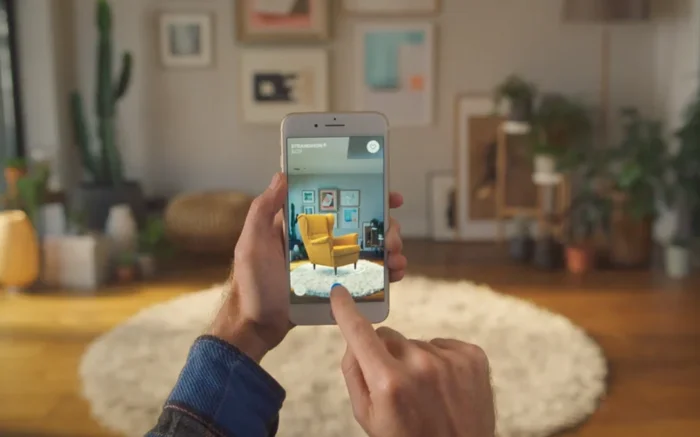
\includegraphics[width=0.9\textwidth]{images/ar_scene_reconstruction.png}
	\captionof{figure}{Ví dụ về ứng dụng AR. Thiết bị sử dụng camera để tái tạo một lưới 3D của căn phòng một cách hợp lý.}
	\label{fig:ar_scene_reconstruction}
\end{center}
% Keyword gợi ý: ar scene reconstruction, augmented reality 3d mesh

\subsection{Triển khai tại Biên (Edge Deployment)}
\label{subsec:edge_deployment}
Cả robot và các thiết bị AR/VR đều là các hệ thống tại biên (edge systems). Việc triển khai các mô hình thị giác mạnh mẽ trên các thiết bị này là một thách thức lớn về mặt kỹ thuật, đòi hỏi sự tối ưu hóa trên toàn bộ pipeline.

\subsubsection{Yêu cầu Cốt lõi}
\label{subsubsec:edge_requirements}
\begin{itemize}
	\item \textbf{Độ trễ thấp (Low Latency):} Phản hồi phải gần như tức thời. Một robot không thể đợi nửa giây để nhận ra một vật cản; một ứng dụng AR không thể có độ trễ giữa chuyển động của người dùng và cập nhật của thế giới ảo.
	\item \textbf{Hiệu quả Năng lượng (Power Efficiency):} Hầu hết các thiết bị biên đều hoạt động bằng pin. Các thuật toán phải được tối ưu hóa để giảm thiểu mức tiêu thụ năng lượng.
	\item \textbf{Dấu chân Bộ nhớ Nhỏ (Small Memory Footprint):} Kích thước của mô hình và bộ nhớ RAM cần thiết trong quá trình suy luận phải đủ nhỏ để vừa với tài nguyên hạn chế của thiết bị.
\end{itemize}

\subsubsection{Các Kỹ thuật Tối ưu hóa}
\label{subsubsec:edge_optimization_techniques}
Để đáp ứng các yêu cầu trên, một loạt các kỹ thuật tối ưu hóa được áp dụng sau khi mô hình đã được huấn luyện:
\begin{description}
	\item[Kiến trúc Hiệu quả:] Sử dụng các kiến trúc được thiết kế đặc biệt cho các thiết bị biên, như \textbf{MobileNetV3}, \textbf{EfficientNet-Lite}, hoặc các biến thể Transformer nhỏ gọn như \textbf{MobileViT}.
	\item[Nén Mô hình (Model Compression):]
	\begin{itemize}
		\item \textbf{Lượng tử hóa (Quantization):} Chuyển đổi các trọng số và phép tính từ dấu phẩy động (FP32) sang các định dạng có độ chính xác thấp hơn như số nguyên 8-bit (INT8).
		\item \textbf{Cắt tỉa (Pruning):} Loại bỏ các kết nối hoặc các bộ lọc không quan trọng trong mạng.
		\item \textbf{Chưng cất Tri thức (Knowledge Distillation):} Huấn luyện một mô hình nhỏ để bắt chước hành vi của một mô hình lớn.
	\end{itemize}
	\item[Các Framework Triển khai Chuyên dụng:] Sử dụng các bộ công cụ như \textbf{NVIDIA TensorRT}, \textbf{Apple CoreML}, \textbf{TensorFlow Lite (TFLite)}, hoặc \textbf{Qualcomm SNPE} để biên dịch và tối ưu hóa mô hình cho một phần cứng cụ thể (GPU, NPU, DSP), tận dụng tối đa khả năng tăng tốc của nó.
\end{description}

\subsection{Kết luận: Cầu nối giữa AI và Thế giới Thực}
\label{subsec:robotics_ar_edge_conclusion}
Thị giác máy tính cho robot, AR/VR, và các thiết bị biên không chỉ là một nhánh ứng dụng; nó là bài kiểm tra cuối cùng, là nơi "lý thuyết gặp thực tế". Đây là nơi các mô hình AI phải đối mặt với sự phức tạp, sự không chắc chắn, và các ràng buộc vật lý của thế giới thực.

Sự hội tụ của các mô hình nền tảng mạnh mẽ (cung cấp khả năng nhận thức tổng quát), các kiến trúc hiệu quả (như CNN/ViT lai), và các kỹ thuật tối ưu hóa triển khai tiên tiến đang thúc đẩy một làn sóng mới của các ứng dụng thông minh. Trong tương lai gần, chúng ta sẽ thấy ngày càng nhiều các hệ thống có khả năng nhận thức và tương tác với môi trường một cách liền mạch, từ những con robot có thể hỗ trợ con người trong các công việc hàng ngày, đến những chiếc kính AR có thể biến thế giới xung quanh chúng ta thành một không gian thông tin tương tác.

\section*{Tài liệu tham khảo}
\begin{itemize}
	\item[1] Mur-Artal, R., Montiel, J. M. M., \& Tardós, J. D. (2015). ORB-SLAM: a versatile and accurate monocular SLAM system. \textit{IEEE transactions on robotics}, 31(5), 1147-1163. (Một trong những hệ thống Visual SLAM kinh điển và có ảnh hưởng nhất).
	\item[2] Mehta, S., \& Rastegari, M. (2021). Mobilevit: light-weight, general-purpose, and mobile-friendly vision transformer. \textit{arXiv preprint arXiv:2110.02178}. (Giới thiệu MobileViT, một kiến trúc lai hiệu quả cho thiết bị di động).
	\item[3] Sandler, M., Howard, A., Zhu, M., Zhmoginov, A., \& Chen, L. C. (2018). Mobilenetv2: Inverted residuals and linear bottlenecks. In \textit{CVPR}. (Giới thiệu MobileNetV2, một kiến trúc nền tảng cho các mạng CNN hiệu quả).
	\item[4] Liu, Z., Lin, Y., Cao, Y., Hu, H., Wei, Y., Zhang, Z., ... \& Guo, B. (2021). Swin transformer: Hierarchical vision transformer using shifted windows. In \textit{ICCV}. (Swin Transformer, với cấu trúc phân cấp, rất phù hợp cho các tác vụ dày đặc trong robot và AR).
	\item[5] Kerbl, B., Kopanas, G., Leimkühler, T., \& Drettakis, G. (2023). 3d gaussian splatting for real-time radiance field rendering. \textit{ACM Transactions on Graphics (TOG)}. (Công nghệ nền tảng cho các ứng dụng AR/VR thời gian thực).
	\item[6] Driess, D., et al. (2023). Palm-e: An embodied multimodal language model. \textit{arXiv preprint arXiv:2303.03378}. (Một ví dụ về việc tích hợp LVLMs vào robot để điều khiển bằng ngôn ngữ tự nhiên).
\end{itemize}